% !TEX program = xelatex

\documentclass[letterpaper,10pt,twoside]{report}
\usepackage{amsmath, amssymb, amsfonts, amsthm, bm, tensor}
\usepackage{mathtools, mathrsfs}
\usepackage{graphicx, fancyhdr}
\usepackage{xcolor, listings, hyperref, lastpage, doi, url}
\usepackage[left=1.in, right=1.in, top=1.5in, bottom=1.in, headheight=42pt]{geometry}
\usepackage{booktabs, siunitx}
\usepackage[style=authoryear, backend=biber, natbib=true]{biblatex}
\setlength\bibitemsep{1.5\itemsep}

%%%%%%%%%%%%%%%%%%%%%%%%%%%%%%%%%%
% Setup the header and the footer
% first I'll make some colors
\definecolor{gugray}{HTML}{666666}
\definecolor{gured}{HTML}{9a3b26}
\definecolor{gublue}{RGB}{0,63,114}

% Add a rule across the top and bottom
\renewcommand{\headrule}{{\color{gugray}%
  \hrule width\headwidth height\headrulewidth \vskip-\headrulewidth}}
\renewcommand{\footrule}{{\color{gugray}%
  \vskip-\footruleskip\vskip-\footrulewidth%
\hrule width\headwidth height\footrulewidth\vskip\footruleskip}}
\renewcommand{\headrulewidth}{1.0pt}
\renewcommand{\footrulewidth}{1.0pt}

\pagestyle{fancy}

% specify what to put in each header box
\lhead{\color{gublue}}
\chead{\color{gublue}ENSC 481}
\rhead{}
\lfoot{}
\cfoot{\color{gugray}\thepage}
\rfoot{}


%%%%%%%%%%%%%%%%%%%%%%%%%%%%%%%%%%
% setup Listings Package from Matlab:
\definecolor{matcolor_comment}{rgb}{0.13333333,0.54509804,0.13333333}
\definecolor{matcolor_keyword}{rgb}{0,0,1}
\definecolor{matcolor_strings}{rgb}{0.62745098,0.12549020,0.94117647}
\lstset{language=Matlab,
frame=ltrb,framesep=5pt,basicstyle=\ttfamily\normalsize,
numbers=left,
identifierstyle=\color{black},
keywordstyle=\color{matcolor_keyword},
stringstyle=\color{matcolor_strings},
commentstyle=\color{matcolor_comment}}

%%%%%%%%%%%%%%%%%%%%%%%%%%%%%%%%%%
% These are some macros to make vectors/matrices Dr Fitz style
\providecommand\Vec{}
%\renewcommand{\Vec}[1]{ \vec{#1} }
\renewcommand{\Vec}[1]{ \bm{#1} }
% Unit vector
\newcommand{\uVec}[1]{ \hat{\bm{#1}} }
% 2nd order Tensor
\newcommand{\Ten}[1]{ \bm{#1} }
% 4th order Tensor
\newcommand{\TenF}[1]{ \bm{\mathfrak{#1}} }
% Colum Vector
\newcommand{\Col}[1]{ \bm{\mathsf{#1}} }
% Matrix
\newcommand{\Mat}[1]{ \bm{ \mathsf{ #1 }} }


%%%%%%%%%%%%%%%%%%%%%%%%%%%%%%%%%%
% Start the document
\begin{document}

\chapter{Chapter title}

%--------------------------------------------------------------
\section{Section title}
Welcome to \LaTeX!

%--------------------------------------------------------------
\subsection{Math}
In the Matlab example I plot the following function
\begin{align}
    f(t) = \sin\left( 2\pi \left( \frac{c}{2}t^2 + f_0 t \right) \right)
\end{align}

%--------------------------------------------------------------
\subsection{Graphics}

I'm using the \texttt{graphicx} package to add a pdf into this example.
We can see the results in Figure \ref{fig:func1}.
The code to produce this figure is provided in \S\ref{sec:code}.

\begin{figure}[h!] % the [h!] means "put it here and don't float it around"
    \centering
    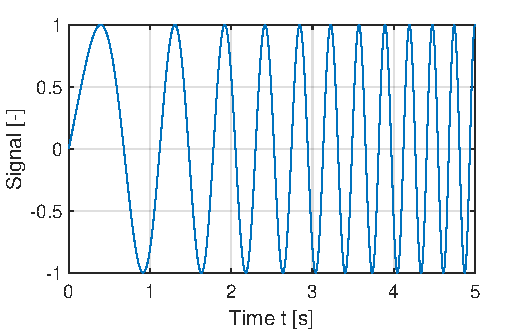
\includegraphics[scale=1]{chirp}
    \caption{This a cool function}
    \label{fig:func1}
\end{figure}

\subsection{Some notation}

To demonstrate some of the flexability of the math fonts I've written out Table \ref{tab:notation}.
It also shows building a table using the \texttt{tabular} package.

\vspace{24pt}
\begin{table}[h!]
   \centering
   \caption{Summary of the notation convention for math quantities}
   \label{tab:notation}
\begin{tabular}{lccl}
  \toprule
  \textbf{Quantity} & \textbf{Group} & \textbf{Symbols} & \textbf{Notes}\\
  \midrule
  scalar & $\mathbb{R}$, $\mathbb{C}$, or $\mathbb{Z}$ & $a,\, b,\, c,\, \ldots$ & italics, upper and lower case \\
          &                                             & $\alpha,\, \beta,\, \gamma ,\, \ldots$ & Greek and Latin \\
  \midrule
  vector (order 1 tensors) & $\mathbb{E}^3$ &  $\Vec{a},\, \Vec{b},\, \Vec{c},\, \ldots$ & lower case, bold italics \\
  2${}^\text{nd}$ order tensor & $\text{Lin}\coloneqq \mathcal{L}\left(\mathbb{E}^3,\mathbb{E}^3 \right)$ & $\Ten{A},\, \Ten{B},\, \Ten{C} \ldots$ & upper case, bold italics \\
  4${}^\text{th}$ order tensor & $\mathcal{L}\left(\text{Lin},\text{Lin}\right)$ & $\TenF{A},\, \TenF{B},\, \TenF{C},\, \ldots$ & upper case, bold Fraktur \\
  \midrule
  $n$--tuple & $\mathbb{R}^n$ & $\Col{a},\,\Col{b},\,\Col{c},\, \ldots$ & lower case, bold, sans serif \\
  matrix & $\mathbb{R}^{n\times m}$ & $\Col{A},\,\Col{B},\,\Col{C},\, \ldots$ & upper case, bold, sans serif \\
  \bottomrule
\end{tabular}
\end{table}

%--------------------------------------------------------------
\section{Further reading}
Some more topics to look into include
\begin{itemize}
    
    \item Making \href{https://en.wikibooks.org/wiki/LaTeX/Tables}{tables}.

    \item Managing citations and a bibliography\footnote{This is a nice article \url{https://www.overleaf.com/learn/latex/bibliography_management_with_bibtex}}
    
    \item Working with more math

\end{itemize}


%--------------------------------------------------------------
\section{Code Example}
\label{sec:code}

\lstinputlisting[language=Matlab]{make_figure.m}

\end{document}